\section{Poisson equation in one dimension}
\label{task_1}

In this section, we will solve the one-dimensional Poisson equation
\begin{equation}
\pd[2]{u}{x} = f(x) \qquad (0 < x < 1)
\label{poisson_equation}
\end{equation}
subject to a source term $f(x)$ and different combinations of Dirichlet and Neumann boundary conditions at $x = 0$ and $x = 1$.
First, we will solve it with finite difference methods of first and second order on a uniform grid.
Finally, we solve it on a non-uniform grid and investigate how adaptive mesh refinement (AMR) can be used to obtain accurate solutions by distributing fewer points more cleverly along the grid.

\subsection{Analytical solution}

One way to express the analytical solution is to simply integrate \cref{poisson_equation} twice to get
\begin{equation}
\begin{split}
u(x) &= C_1 + \int^x \dif x' u_x(x') \\
     &= C_1 + \int^x \dif x' \left(C_2 + \int^{x'} \dif x'' u_{xx}(x'')\right) \\
     &= C_1 + C_2 x + \int^x \dif x' \int^{x'} \dif x'' f(x''),
\label{poisson_analytical_solution}
\end{split}
\end{equation}
where the constants $C_1$ and $C_2$ are determined from two boundary conditions and the integrals can be done from any lower limit.
Note that this is equivalent to saying that the solution is a sum of the solution to the homogeneous equation $u_{xx} = 0$ and a solution to the inhomogeneous equation $u_{xx} = f(x)$.

Note that if \emph{two} Neumann boundary conditions $u_x(0) = a$ and $u_x(1) = b$ are imposed, then the solution $u(x)$ is unique only up to a constant.
If $u(x)$ is a solution to the boundary value problem defined by \cref{poisson_equation} with $u_x(0) = a$ and $u_x(1) = b$, then also $(u+C)_{xx} = u_{xx}$ in the interior and $(u+C)_x(0) = u_x(0) = a$ on the left boundary, and similarly on the right boundary $x=1$.
It can also be seen by observing that $C_1$ is undetermined when \ref{poisson_analytical_solution} is differentiated.

\subsection{Numerical solution on a uniform grid}
In order to achieve a numerical solution to the problem, we first consider the boundary value problem defined by \cref{poisson_equation}, subject to the boundary conditions
\begin{equation*}
u(0) = a \quad \text{or} \quad u_x(0) = a \qquad \text{and} \qquad u(0) = b \quad \text{or} \quad u_x(1) = b.
\end{equation*}
To solve the equation numerically, we divide the interval $[0, 1]$ into the uniform grid 
\begin{center}
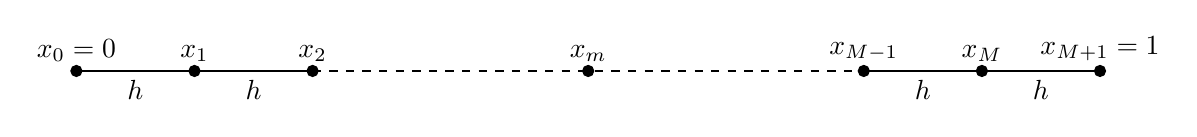
\begin{tikzpicture}
\draw (0,0) -- (3,0);
\draw[dashed] (3,0) -- (10,0);
\draw (10,0) -- (13,0);
\filldraw (0.0,0) circle (2pt) node[anchor=south] {$x_0 = 0$};
\filldraw (1.5,0) circle (2pt) node[anchor=south] {$x_1$};
\filldraw (3.0,0) circle (2pt) node[anchor=south] {$x_2$};
\filldraw (6.5,0) circle (2pt) node[anchor=south] {$x_m$};
\filldraw (10.0,0) circle (2pt) node[anchor=south] {$x_{M-1}$};
\filldraw (11.5,0) circle (2pt) node[anchor=south] {$x_{M}$};
\filldraw (13.0,0) circle (2pt) node[anchor=south] {$x_{M+1} = 1$};
\node[anchor=north] at (0.75, 0) {$h$};
\node[anchor=north] at (2.25, 0) {$h$};
\node[anchor=north] at (10.75, 0) {$h$};
\node[anchor=north] at (12.25, 0) {$h$};
\end{tikzpicture}
\end{center}
of $M+2$ points and step length $h$.
We approximate the second derivative at interior points with the central difference
\begin{equation*}
\pd[2]{u}{x}(x_m) = \frac{u_{m-1}-2u_{m}+u_{m+1}}{h^2} + \Oh(h^2) \qquad (1 \leq m \leq M-1).
\end{equation*}
Discarding terms of $\Oh(h^2)$ and denoting the approximation of the solution $u_m$ as $U_m$, 
we get the finite difference formula
\begin{equation}
\frac{U_{m-1}-2U_{m}+U_{m+1}}{h^2} = f_m \qquad (1 \leq m \leq M-1).
\label{eq:task1-finite-diff-approx}
\end{equation}
To handle the Dirichlet boundary condition $u(0) = a$ at the left edge or $u(1) = b$ at the right edge, we insert the trivial equation
\begin{equation*}
1 \cdot u_0 = a \qquad \text{or} \qquad 1 \cdot u_{M+1} = b.
\end{equation*}
To handle the Neumann boundary condition $u_x(0) = a$ at the left edge or $u_x(1) = b$ at the right edge to second order, we approximate the first derivative to second order with forward or backward differences to get
\begin{equation*}
u_x(0) = \frac{-\frac{3}{2}u_{0}-2u_1-\frac{1}{2}u_{2}}{h} + \Oh(h^2) = b \qquad \text{or} \qquad u_x(1) = \frac{\frac{1}{2}u_{M-1}-2u_M+\frac{3}{2}u_{M+1}}{h} + \Oh(h^2) = b.
\end{equation*}
Writing all these equations in $(M+2) \times (M+2)$-matrix form $AU=b$, we obtain for example with $u(0) = a$ and $u_x(1) = b$
\begin{equation}
\renewcommand{\arraystretch}{1.5} % stretch matrix vertically to make it square
\begin{bmatrix}
1 \\
+1/h^2 & -2/h^2 & +1/h^2 &   \\
  & \ddots & \ddots & \ddots & \\
  &   & +1/h^2 & -2/h^2 & +1/h^2 \\
  &   & +1/2h & -2/h & +3/2h \\
\end{bmatrix}
\begin{bmatrix}
U_0 \\ U_1 \\ \vdots \\ U_M \\ U_{M+1} \\
\end{bmatrix}
=
\begin{bmatrix}
a \\ f(x_1) \\ \vdots \\ f(x_M) \\ b \\
\end{bmatrix}
,
\label{matrix_system}
\end{equation}
where the first and last rows of the matrix generally vary depending on the boundary conditions.

Note that if the numerical solution is subject to two Neumann boundary conditions, the matrix becomes singular and the solution non-unique.
In this case, we impose the additional constraint $U_0 = 0$ by setting all entries in the first column of $A$ to zero.
To handle the singular matrix, we instead find the least-squares solution to the matrix equation. \cite{numpy_lstsq}

\begin{figure}[tb]
	\centering
	\begin{tikzpicture}
		\begin{groupplot}[
			group style={group size=2 by 3,horizontal sep=2cm,vertical sep=2.2cm},
			height=6cm,
			width=0.48\textwidth,
			clip marker paths=true,
      legend style={at={(0.5,+1.2)},anchor=north}, legend columns=-1,
			]
			\nextgroupplot[title={$u(0)=0, \quad u_x(1)=1$},xmode=normal,ymode=normal,xlabel=$x$,ylabel=$u(x)$,legend entries={$u(x)$,$U(x)$}];
			% \addplot [color=black, line width=4pt] table [x=x,y=u] {exercise1/dir_neu.dat};
			% \addplot [color=red, mark=*, mark size=1pt, line width=1pt, each nth point=1] table [x=x,y=U] {exercise1/dir_neu.dat};
			\addplot [color=black, thick] table [x=x,y=u] {exercise1/dir_neu.dat};
			\addplot [color=blue, mark=square*, mark size=1pt, thin] table [x=x,y=U] {exercise1/dir_neu.dat};
			\nextgroupplot[xmode=log,ymode=log,xlabel=$M$,ylabel={$\Ltwoerror{u-U}/\Ltwoerror{u}$},legend entries={$L_2$ (cont.),$L_2$ (disc.)},xmin=5,xmax=2000];
			\addplot [black, dashed, domain=1:3000, samples=2, forget plot] {1.45/(x)^2} node
             [pos=0.47,
               pin={[pin edge={solid}]-95:$\Oh(h^2)$},
               inner sep=0pt] {};
			\addplot [red!75!black, mark=square*] table [x=M,y=cont] {exercise1/dir_neu_err.dat};
			\addplot [red!100!black, mark=*] table [x=M,y=disc] {exercise1/dir_neu_err.dat};

			\nextgroupplot[title={$u(0)=1, \quad u(1)=1$},xmode=normal,ymode=normal,xlabel=$x$,ylabel=$u(x)$];
			\addplot [color=black, thick] table [x=x,y=u] {exercise1/dir_dir.dat};
			\addplot [color=blue, mark=square*, mark size=1pt, thin] table [x=x,y=U] {exercise1/dir_dir.dat};
			\nextgroupplot[xmode=log,ymode=log,xlabel=$M$,ylabel={$\Ltwoerror{u-U}/\Ltwoerror{u}$},xmin=5,xmax=2000];
			\addplot [black, dashed, domain=1:3000, samples=2] {0.10/(x)^2};
			\addplot [red!75!black, mark=square*] table [x=M,y=cont] {exercise1/dir_dir_err.dat};
			\addplot [red!100!black, mark=*] table [x=M,y=disc] {exercise1/dir_dir_err.dat};

			\nextgroupplot[title={$u_x(0)=0, \quad u_x(1)=1/2$},xmode=normal,ymode=normal,xlabel=$x$,ylabel=$u(x)$,scaled ticks=false, tick label style={/pgf/number format/fixed}];
			\addplot [color=black, thick] table [x=x,y=u] {exercise1/neu_neu.dat};
			\addplot [color=blue, mark=square*, mark size=1pt, thin] table [x=x,y=U] {exercise1/neu_neu.dat};
			\nextgroupplot[xmode=log,ymode=log,xlabel=$M$,ylabel={$\Ltwoerror{u-U}/\Ltwoerror{u}$},xmin=5,xmax=2000];
			\addplot [black, dashed, domain=1:3000, samples=2] {3.60/(x)^2};
			\addplot [red!75!black, mark=square*] table [x=M,y=cont] {exercise1/neu_neu_err.dat};
			\addplot [red!100!black, mark=*] table [x=M,y=disc] {exercise1/neu_neu_err.dat};
		\end{groupplot}
	\end{tikzpicture}
	\caption{\label{poisson_numerical_solutions}
		The left plots show analytical solutions $u(x)$ and numerical solutions $U(x)$ with $M=30$ grid points for $u_{xx} = x + \cos{2 \pi x}$ subject to three different boundary conditions.
		The right plots show convergence plots corresponding to the same boundary conditions, where the error is measured with both the a continuous and discrete $L_2$-norm.
	}
\end{figure}

We now apply our method to the boundary value problem with the source function 
\begin{equation*}
f(x) = x + \cos(2 \pi x).
\end{equation*}
Inserting it into \cref{poisson_analytical_solution} and doing the integrals, we get the exact solution
\begin{equation*}
u(x) = C_1 + C_2 x + \frac{1}{3!}x^3 - \frac{1}{4 \pi^2}\cos(2 \pi x)).
\end{equation*}
In \cref{poisson_numerical_solutions}, we present numerical solutions for three different combinations of boundary conditions. 
To the right of each solution plot is the corresponding convergence plot, 
resulting from refinement of the uniform grid. 
The convergence plots show the computed relative errors at varying grid resolution, 
together with the expected convergence rate. 

To find the expected convergence rate, we start by insert the exact solution into the finite difference formula \eqref{eq:task1-finite-diff-approx}. 
This gives rise to an additional term, 
the \textit{local truncation error} $\tau_m$, 
since the equality in the formula does not hold for the exact solution. 
We get that 
\begin{equation}
    \tau_m = \frac{u_{m-1}-2u_m+u_{m+1}}{h^2} - f_m. 
    \label{eq:task1-truncation-error}
\end{equation}
We now Taylor expand the terms around $u_m$, 
and the only difference between the expansion of $u_{m-1} = u(x_m - h)$ and the expansion of $u_{m+1}=u(x_m+h)$, 
is the sign in front of the odd-order terms, which therefore cancel. 
The expansion of the truncation error is thus 
\begin{align*}
    \tau_m & = \frac{1}{h^2}\left(-2u_m + 2u_m + 2\frac{h^2}{2}\partial_x^2 u_m + 2\frac{h^4}{24}\partial_x^4 u_m + \Oh(h^6) \right) - f_m\\
           & = \partial_x^2 u_m + \frac{h^2}{12}\partial_x^4 u_m + \Oh(h^4) - f_m \\
           & = \frac{h^2}{12}\partial_x^4 u_m + \Oh(h^4) \\
           & = \Oh(h^2). 
\end{align*} 

For relating the local error $\tau_m$ to the global error and the expected convergence rate, 
we will for brevity just provide a slightly rough discussion. 
By rearranging \eqref{eq:task1-truncation-error} and subtracting it from equation \eqref{eq:task1-finite-diff-approx}, 
we can express the discretization error $e_m = U_m - u_m$ implicitly by 
\begin{equation*}
    \frac{1}{h^2}\delta^2(u_{m} - U_m) = \frac{1}{h^2}\delta^2e_m = \tau_m. 
\end{equation*}
Defining the vectors $E = [e_1, \dots, e_m]$ and $\tau = [\tau_1, \dots, \tau_m]$, 
we can write this on matrix form so that 
\begin{equation*}
    A'E = \tau. 
\end{equation*}
The matrix $A'$ can be shown to be invertible, 
and for the matrix norms subordinate to both the $L_2$ continuous function norm, and the $l_2$ discrete vector norm, 
one can also show that $\|(A')^{-1}\|$ is bounded. 
This means that 
\begin{equation*}
    \|E\| = \| (A')^{-1} \tau_m \| \leq \| (A')^{-1} \| \cdot \| \tau_m \| = C\|\tau\|. 
\end{equation*}
Thus we can expect that the global error converges as the local truncation error. 

Our approach to handling the boundary conditions is not the only possible approach.
The system of equations is equivalent if we remove the first row and column of $A$ and the first entries in $U$ and $b$, but simultaneously modify the entry $f(x_1) \rightarrow f(x_1) - a/h^2$.
This approach is done in \cite{owren}, for example, and is more consistent with treating $U_0$ as a known variable, since its precise value is defined by the Dirichlet boundary condition.
However, our approach of inserting a trivial equation $1 \cdot U_0 = a$ keeps the matrix dimensions independent of boundary conditions and makes it easier to reason with how the discretized differential operator represented by $A$ operates on the grid point $U_0$ in the same way it operates on all other grid points.

Neumann boundary conditions can also be handled differently.
Instead of approximating the second derivative only on actual grid points, we could approximate it with a fictuous point $x_{-1}$ and a central difference $u_x(0) \approx (U_1 - U_{-1}) / (2 h)$.
Then we could use this together with the central difference $(U_{-1} - 2 U_0 + U_1) / h^2 = f(x_0)$ to eliminate $U_{-1}$.
Eliminating $U_{-1}$, the first equation becomes $(U_1 - U_0) / h = a + h f(x_0) / 2$, so the boundary condition could be handled by setting the first row to $[-1/h, +1/h, 0, \dots]$ and modifying the first entry in $b$ to $a \rightarrow a + h f(x_0) / 2$.
This would also be second order, and would allow us to use the same stencil also at $x_0$, but we would then have to pay the price of modifying the right side of the matrix equation in an unnatural way.
This approach is also done in \cite{owren}.




\subsection{Adaptive numerical solution on a non-uniform grid}

\label{ex1_amr_section}

We will now demonstrate how the numerical solution can be generalized to a non-uniform grid with $x_i - x_{i-1} \neq \text{const}$.
Then we will attempt to make the numerical solution as good as possible using as few grid points as possible, by placing points tighter where the solution varies rapidly.

To derive a nonuniform stencil for the second derivative at $x_m$, we proceed similarly to the uniform stencil.
First approximate one derivative by stepping halfway left and right, landing at $x_{m-1/2}$ and $x_{m+1/2}$.
Then we approximate another derivative by stepping halfway to the sides again, landing at $x_{m-1}$, $x_{m}$ and $x_{m+1}$.
This yields
\newcommand\nonuniformstencil[4]{\frac{2}{x_{#4}-x_{#2}} \left( \frac{#1_{#4}-#1_{#3}}{x_{#4}-x_{#3}} - \frac{#1_{#3}-#1_{#2}}{x_{#3}-x_{#2}} \right)}
\begin{equation*}
\begin{split}
%\dpd[2]{u}{x}(x_m) &\approx \frac{u_x(x_m+\frac{x_{m+1}-x_m}{2}) - u_x(x_m-\frac{x_m-x_{m-1}}{2})}{(x_m + \frac{x_{m+1}-x_m}{2}) - (x_m - \frac{x_m-x_{m-1}}{2})} \\
%                   &=       \frac{2}{x_{m+1} - x_{m-1}} \left( u_x(x_m+\frac{x_{m+1}-x_m}{2}) - u_x(x_m-\frac{x_m-x_{m-1}}{2}) \right) \\
%                   &\approx \frac{2}{x_{m+1} - x_{m-1}} \left( \frac{u(x_{m+1})-u(x_m)}{x_{m+1}-x_m} - \frac{u(x_m)-u(x_{m-1})}{x_m-x_{m-1}} \right) \\
u''_m &\approx \frac{u'_{m+1/2} - u'_{m-1/2}}{x_{m+1/2}-x_{m-1/2}}
      % \approx \frac{1}{x_{m+1/2}-x_{m-1/2}} \left( \frac{u_{m+1}-u_m}{x_{m+1}-x_m} - \frac{u_m-u_{m-1}}{x_m-x_{m-1}} \right) \\
      %&=       \frac{2}{x_{m+1}-x_{m-1}} \left( u'_{m+1/2} - u'_{m-1/2} \right) \\
      %&\approx \frac{2}{x_{m+1}-x_{m-1}} \left( \frac{u_{m+1}-u_m}{x_{m+1}-x_m} - \frac{u_m-u_{m-1}}{x_m-x_{m-1}} \right) \\
	  \approx \nonuniformstencil{u}{m-1}{m}{m+1}.\\
\end{split}
\label{amr_stencil}
\end{equation*}

\newcommand\hleft{x_m-x_{m-1}}
\newcommand\hright{x_{m+1}-x_m}
\newcommand\hfull{x_{m+1}-x_{m-1}}
Assuming Dirichlet boundary conditions, the nonzero entries of $A$ (indexed from zero) becomes
\begin{equation*}
\begin{aligned}
A_{0,0} &= A_{M+1, M+1} = 1
\qquad
&A_{m,m-1}       &= \frac{2}{\hfull} \frac{1}{\hleft} \\
A_{m,m  }       &= \frac{-2}{\hfull} \left( \frac{1}{\hleft} + \frac{1}{\hright} \right)
\qquad
&A_{m,m+1}       &= \frac{2}{\hfull} \frac{1}{\hright}.\\
\end{aligned}
\end{equation*}
The job is then once again to solve the system $A U = b$.
Note that the stencil reduces to the one in \cref{matrix_system} when $\hleft = \hright = h$, as it should.

To do adaptive mesh refinement, we will
\begin{enumerate}
\item Start with a coarse uniform grid, such as $[x_0, x_1] = [0, 1]$.
\item Wisely choose \emph{one} grid interval $[x_m, x_{m+1}]$ based on some strategy.
\item Split the interval in half by inserting a new point at $(x_m + x_{m+1}) / 2$.
\item Repeat step 2 and 3 until the grid has the desired resolution.
\end{enumerate}
We will compare three different strategies for selecting the grid interval:
\begin{enumerate}
\item \textbf{Error strategy:} Select the interval $[x_m, x_{m+1}]$ with the largest error
\begin{equation*}
\int_{x_m}^{x_{m+1}} \dif x |u(x) - U(x)|, \qquad \text{where} \,\, U(x) = U_m + \frac{x - x_m}{x_{m+1} - x_m} \left( U_{m+1} - U_m \right)
\end{equation*}
is a linearly interpolated numerical solution on the \emph{current} grid and $u(x)$ is the exact solution.
This strategy requires knowledge of the exact solution $u(x)$ and solving the system numerically before each splitting.

\item \textbf{Truncation error strategy:} Select the interval $[x_m, x_{m+1}]$ with the largest absolute truncation error
\begin{equation*}
\left| \nonuniformstencil{u}{m}{m+1/2}{m+1} - f(x_m) \right|,
\end{equation*}
upon insertion of a middle point $x_{m+1/2} = (x_m + x_{m+1})/2$, where $u(x)$ is the exact solution.
This strategy also requires knowledge of the exact solution $u(x)$, but does not rely on intermediate computations of the numerical solution.

\item \textbf{Source strategy:} Select the interval $[x_m, x_{m+1}]$ with the largest ``absolute source''
\begin{equation*}
\int_{x_m}^{x_{m+1}} \dif x |f(x)|.
\end{equation*}
In physical applications, $f(x)$ is typically mass density or charge density. 
The idea is to refine intervals on which there is much mass or charge, as the solution is expected to vary faster there.
This splitting strategy requires neither knowledge of the exact solution or the numerical solution, only on the source function $f(x)$, as is typically the case in practice.
\end{enumerate}

% In \cref{amr_error_evolution}, we demonstrate how the grid and the numerical solution evolves as the grid $[0, 1/2, 1]$ with $M = 3$ is refined to $M = 25$.
% In \cref{amr_convergence_plot}, we show how the convergence of the three different AMR strategies compares to the second order UMR method.
% The error strategy and truncation error strategy makes AMR comparable to second order UMR, even though \ref{amr_stencil} has lower order!
% Moreover, the error-based AMR even produces a lower error than the UMR solution for select grids, and seems to do so in a periodic manner as the grid size $M$ increases!

In \cref{amr_error_evolution}, we demonstrate how the initial grid $[0, 0.5, 1]$ and the numerical solution $U(x)$ evolves through adaptive refinement with the error strategy.
Observe how the refinement concentrates on resolving critical areas of the solution near the peak and the inflection points.

In \cref{amr_convergence_plot}, we compare the convergence of the three adaptive refinement strategies to the $\Oh(h^2)$-convergence of uniform refinement on the same problem.
The error strategy requires knowledge of the exact solution and intermediate computations, but in return it is the most effective strategy.
The source strategy requires neither, but is also the least effective strategy.
We can say that the more knowledge of the exact solution and intermediate computations, the greater the accuracy.

Note that the errors are not strictly decreasing with each refinement $M \rightarrow M+2$.
In particular, the error from the error strategy exhibits an oscillating pattern for $M \geq 32$.
This is a weakness of refining only \emph{exactly} two symmetric intervals for each refinement.
An alternative method is to refine \emph{multiple} intervals at every refinement step using a criterion that splits not only the interval with the largest error, but all intervals with error above some reference error.
This procedure removes our control over the exact number of intervals, but in return gives us control over the maximal acceptable error on any interval.
In \cref{fem_amr_section}, we will improve our AMR strategy exactly in this way.
The effect is that the oscillating pattern is eliminated and that the error decreases strictly with each refinement step.
This will be equivalent to jumping directly from one local minimum in the oscillation to the next.

\begin{figure}[tb]
\centering
\begin{tikzpicture}
\begin{groupplot}[
	group style={group size=3 by 4,horizontal sep=0.25cm,vertical sep=0.25cm},
	height=5.9cm, width=5.9cm,
	xmin=0, xmax=1, ymin=0, ymax=1.2, 
	xtick={0, 0.5, 1},
	legend style={at={(0.5,+1.2)},anchor=north}, legend columns=-1,
]
\pgfplotsinvokeforeach{3,5,7,9,11,13,15,17,19,21,23,25} {
\ifthenelse{#1>21}{
	\nextgroupplot[xlabel=$x$,yticklabels={,,},xtick=data,xticklabels={,,}, extra x ticks={0, 1}];
}{\ifthenelse{\equal{#1}{21}}{
	\nextgroupplot[xlabel=$x$,xtick=data,xticklabels={,,}, extra x ticks={0, 1}];
}{\ifthenelse{\equal{#1}{3} \OR \equal{#1}{9} \OR \equal{#1}{15}}{
	\nextgroupplot[xticklabels={,,},xtick=data];
}{\ifthenelse{\equal{#1}{5}}{
	\nextgroupplot[xticklabels={,,},yticklabels={,,},xtick=data,legend entries={,{$u(x) = \exp(-(x-1/2)^2/0.1)$},$U(x)$}];
}{
	\nextgroupplot[xticklabels={,,},yticklabels={,,},xtick=data];
}}}}
\addplot table [x=x, y expr=-1] {exercise1/amre_M#1.dat}; % hidden dummy plot, just go get the ticks
% \addplot [line width=5pt, black, mark=none, domain=0:1   ] {exp(-(x-0.5)^2/0.1)};
% \addplot [line width=1pt, red  , mark=*   , mark size=1pt] table [x=x, y=U] {exercise1/amre_M#1.dat};
\addplot [black, mark=none,    domain=0:1, thick, samples=100] {exp(-(x-0.5)^2/0.1)};
\addplot [blue , mark=square*, mark size=1pt, thin] table [x=x, y=U] {exercise1/amre_M#1.dat};
\node at (0.5, 0.5) {$M=#1$};
}
\end{groupplot}
\end{tikzpicture}
\caption{
	\label{amr_error_evolution}
	During adaptive mesh refinement (AMR) with the error strategy (strategy number 1), the interval with the largest error $\int \dif x |u(x) - U(x)|$ is split in half.
	Here, $u(x) = \exp(-(x-1/2)^2/0.1)$ is the symmetric solution to whichever Poisson equation has $f(x) = u_{xx}$ on $x \in [0, 1]$.
	Symmetry is imposed numerically by also adding the point $1 - x$ to the grid whenever a point $x \neq 1/2$ is added.
}
\end{figure}

\begin{figure}[tb]
\centering
\begin{tikzpicture}
  \begin{loglogaxis}[
	width=16.5cm, height=12cm,
	xlabel=$M$, ylabel=$\Ltwoerror{u - U}/\Ltwoerror{u}$,
	log basis x=2, xticklabel=\pgfmathparse{2^\tick}\pgfmathprintnumber\pgfmathresult,
	grid=major,
	xmin=1.9, xmax=360,
	legend style={at={(0.5,+1.13)},anchor=north}, legend cell align=left,
	transpose legend, legend columns=2, legend entries={
		{UMR (disc.)},
		{UMR (cont.)},
		{AMR err. (disc.)},
		{AMR err. (cont.)},
		{AMR trunc. err. (disc.)},
		{AMR trunc. err. (cont.)},
		{AMR source (disc.)},
		{AMR source (cont.)}
	}, cycle list={
		% {black, densely dashed, line width=1.0pt, mark=*, mark size=1.3pt},
		% {black, solid,  line width=1.0pt, mark=*, mark size=1.3pt},
		% {red,   densely dashed, line width=1.0pt, mark=*, mark size=1.3pt},
		% {red,   solid,  line width=1.0pt, mark=*, mark size=1.3pt},
		% {blue,  densely dashed, line width=1.0pt, mark=*, mark size=1.3pt},
		% {blue,  solid,  line width=1.0pt, mark=*, mark size=1.3pt},
		% {green, densely dashed, line width=1.0pt, mark=*, mark size=1.3pt},
		% {green, solid,  line width=1.0pt, mark=*, mark size=1.3pt},
		{red,            solid, mark=x, mark size=1.2pt},
		{red,            solid, mark=o, mark size=1.2pt},
		{cyan!60!black,  solid, mark=x, mark size=1.2pt},
		{cyan,           solid, mark=o, mark size=1.2pt},
		{green!60!black, solid, mark=x, mark size=1.2pt},
		{green,          solid, mark=o, mark size=1.2pt},
		{yellow!60!black,solid, mark=x, mark size=1.2pt},
		{yellow,         solid, mark=o, mark size=1.2pt},
	},
]
    \addplot [black, dashed, domain=1:400, samples=2, forget plot] {1.8/x^2} node
             [pos=0.31,
               pin={[pin edge={solid}]-100:$\Oh(h^2)$},
               inner sep=0pt] {};
\pgfplotsinvokeforeach{UMR,AMRE,AMRT,AMRS} {
\addplot table [x=#1-M,y=#1-ED] {exercise1/amr_errors.dat};
\addplot table [x=#1-M,y=#1-EC] {exercise1/amr_errors.dat};
% \draw (+5,0) node {a} -- (+6,2) node {b};
}
\end{loglogaxis}
\end{tikzpicture}
\caption{
	\label{amr_convergence_plot}
	Comparison between the convergence of the numerical solution $U(x)$ with uniform mesh refinement (UMR) and adaptive mesh refinement (AMR) on the problem $u_{xx} = f(x)$ on $x \in [0,1]$ with analytical solution $u(x) = \exp(-(x-1/2)^2/0.1)$.
	The adaptive refinement is done using three different strategies that subdivide the interval with the largest absolute error $|u-U|$, largest truncation error $Lu - f(x)$ (where $L \approx \partial^2 / \partial x^2$ is the discretized differentiation operator) or largest amount of source $\int \dif x |f(x)|$.
	Errors $\Vert u - U \Vert_2$ are measured with the continuous and discrete $L_2$-norm.
    Note that a cross inside a circle means that the discrete and continuous error measurements agree.
}
\end{figure}
